\chapter{Introduction and Background}

% \begin{quote}
% \textit{This will be the introduction}
% \end{quote}

%%%%%%%%%%%%%%%%%%%%%%%%%%%%%%%%%5
% Gneral Introduction, some talkson how deep generative mdoels are cool goes here
%%%%%%%%%%%%%%%%%%%%%%%%%%%%%%%%%5
In recent years, deep learning has seen significant advances, particularly in the field of generative models. Two of the most successful applications of Deep Generative Models (DGMs) are natural language processing and computer vision. In natural language processing, Large Language Models (LLMs), which usually constitute autoregressive generative models~\citep{graves2013generating} with a transformer-based architecture~\citep{vaswani2017attention}, have demonstrated impressive text generation capabilities~\citep{brown2020language,chowdhery2023palm}. They have produced long and coherent texts across various contexts and gained popularity in the form of chat bots~\citep{achiam2023gpt}. In computer vision, diffusion models are achieving impressive results in generating photorealistic images~\citep{dhariwal2021diffusion} and videos~\citep{ho2022video}.

% Bayesian inference and human learning \cite{xu2007word}

Practically, modeling the probability distribution of the data offers two main functionalities to the underlying model: sampling and likelihood estimates. A lot of attention is paid to the sampling functionality, as it can be used to produce completely novel datapoints, e.g. images that look like real ones but were not observed by the model during training. Furthermore, conditional sampling from the distribution can be used to provide forecast or prediction in the situation when only part of the variables is observed. Access to the likelihood, if present, might also offer many benefits. This includes, but is not limited to, the estimation of uncertainty and the detection of out-of-distribution \cite{havtorn2021hierarchical, kadavath2022language}, as well as handling the missing data \cite{mattei2019miwae} and anomalies \citep{an2015variational}.

Despite enormous successes, many challenges still remain in the field of deep generative modeling~\citep{manduchi2024challenges}. The present thesis focuses on one type of generative models, namely, Latent Variable Generative Models (LVMs). We consider two general aspects in which deep LVMs can be improved. The first aspect is presented in Part~\ref{part:1} of the thesis and it concerns the choice of the prior distribution and the way it affects model performance in the different scenarios. The second aspect covered in Part~\ref{part:2} focuses on the various properties of the resulting latent representations, which can be especially important for the downstream applications of the generative models. 

In this chapter, we discuss all the background crucial for understanding the contributions of the thesis and lay out the research questions. 


%%%%%%%%%%%%%%%%%%%%%%%%%%%%%%%%%5
% Main Seciton: Generative models Definition
%%%%%%%%%%%%%%%%%%%%%%%%%%%%%%%%%5
\section{Deep Generative Modeling}
We formulate Deep Generative Modeling as a problem of density estimation and deep neural network parametrization. 
The task is to model a distribution of the random variable $\rvx$ given a finite set of independent and identically distributed (\textit{iid}) random samples $\{x_n\}_{n=1}^N$. 
We will denote this finite set of samples as an empirical data distribution $p_e(\rvx) = \frac1N \sum_n \delta\left(\rvx - x_n\right)$. 
There are three components of the model that need to be specified:
\begin{itemize}
\item Probabilistic model. \newline 
The probabilistic model $p_{\theta}(\rvx)$\footnote{
	We use $p_{\theta}(\rvx)$ to denote probability density function of random variable $\rvx$, which is defined by (possibly unknown) parameters $\theta$. 
}.
formalizes the assumption about the generative process of the observed data. 
We seek to have flexible and expressive model to capture complex dependencies in the observed data, while as the same time keeping the method scalable.


\item Parametrization.\\
In deep generative models, the probabilistic model from above is parameterized by the deep neural network. 
The choice of architecture depends on the type of data and should respect any constraints implied by the probabilistic framework (e.g. we expect variance of the distribution to be always positive).

\item Learning algorithm. \\
Finally, one has to choose how to tune unknown parameters $\theta$. The goal is to make sure that $p_{\theta}(\rvx)$ approximates a true data distribution for which only a finite number of samples is observed. For this purpose, we will formulate learning as an optimization problem and solve it using gradient-based methods. 
\end{itemize}


% This thesis focuses on the first component. \todo{Elaborate what exactly or move somewhere}
%%%%%%%%%%%%%%%%%%%%%%%%%%%%%%%%%5
% Types of generative models
%%%%%%%%%%%%%%%%%%%%%%%%%%%%%%%%%5
\section{Generative Models Zoo}\label{sec:gen_zoo}
Deep generative models are usually differentiated by the probabilistic model. 
There are multiple ways in which these models can be grouped. In this chapter, we chose to distinguish the models with prescribed and implicit density \citep{diggle1984monte}. In the former case, the density function can be evaluated at least up to a normalization constant, while in the latter case only the sampling procedure from the distribution is defined. 
In Figure \ref{fig:into_model_types} we schematically present the dichotomy with the examples of modern deep generative models given for each type.

This thesis contributes to the field of prescribed density models with auxiliary variables. To put the work in a more broad context, we will now discuss different types of prescribed density generative models.

\begin{figure}[t]
\begin{tikzpicture}[
node distance=1.5cm and 2cm,
box/.style={rectangle, draw, rounded corners, text centered, text width=4cm, minimum height=1cm, fill=blue!10},
example/.style={rectangle, draw=none, text centered, rounded corners, text width=4cm, minimum height=0.5cm,fill=green!10},
arrow/.style={->, thick, >=Stealth}
]

% Main block at the top center
\node[box, fill=orange!20] (dgms) {Generative Model};

% Subcategories in one horizontal line below the main block
\node[box, below=of dgms, xshift=-3cm, text width=3.5cm] (full) {Prescribed density};
\node[box, below=of dgms, xshift=3cm, text width=3.5cm] (implicit) {Implicit density\\ $\tilde{\rvx} \sim p_{\theta}(\rvx)$};
\node[example, below=0.1cm of implicit, text width=3.5cm] (impl-x) {GAN};
%% Arrows connecting main block to subcategories
\draw[arrow] (dgms) -- (implicit);
\draw[arrow] (dgms) -- (full);


%\node[example, below=0cm of full, text width=4cm] (full-x) {Normalizing Flows};
\node[box, below=of full, xshift=-2cm, text width=3.5cm] (tractable) {Fully Tractable \\ $p_{\theta}(\rvx)$};
\node[box, below=of full, xshift=2cm, text width=3.5cm] (norm) {Unnormalized \\ $ p_{\theta}(\rvx) \propto f_{\theta}(\rvx) $};
\node[box, below=of full, xshift=6.2cm, text width=3.9cm] (aux) {Auxiliary Variables \\ $p_{\theta}(\rvx) = \int p_{\theta}(\rvx| \rvz)p_{\theta}(\rvz)d\rvz$};
\draw[arrow] (full) -- (tractable);
\draw[arrow] (full) -- (norm);
\draw[arrow] (full) -- (aux);

\node[example, below=0.1cm of tractable, text width=3.5cm] (tractable-x) {Normalizing Flow};
\node[example, below=0.1cm of norm, text width=3.5cm] (norm-x) {Energy-based Model};
\node[example, below=0.1cm of aux, text width=3.9cm] (aux-x) {VAE, Diffusion Models};

%\node[box, below=of aux, xshift=-2cm, text width=3.5cm] (latent) {Latent \\ $ p(\rvz) $};
%\node[box, below=of aux, xshift=2cm, text width=3.5cm] (observed) {Non-latent \\ $q(\rvz|\rvx){}$};
%\draw[arrow] (aux) -- (latent);
%\draw[arrow] (aux) -- (observed);

\end{tikzpicture}
\caption{Different types of generative models based on the underlying probabilistic model.}
\label{fig:into_model_types}
\end{figure}


\subsection{Fully Tractable Likelihood}
\textit{Normalizing flow}\footnote[][]{\citet{papamakarios2021normalizing} provide a comprehensive review and details on how to construct normalizing flows.} is an example of a generative model with fully tractable likelihood. Here, the distribution of interest is produced by pushing a simple base distribution $\pi(\cdot)$ through a bijective transformation $f_{\theta}(\cdot)$. This allows to compute the likelihood exactly using change of variables formula:
\begin{equation}\label{eq:intro_nf}
    p_{\theta}(\rvx) = \pi(f^{-1}_{\theta}(\rvx)) \left|\text{det}\mJ_{f_{\theta}}  \right|^{-1}.
\end{equation}
These models allow for fast sampling and exact likelihood calculations. However, the bijectivity requirement introduces a constraint on the parameterization and may influence the expressivity of the model. 

Another way to define a fully tractable probabilistic model over a high dimensional input $\rvx$ is to use the product rule of probability, which gives rise to \textit{Autoregressive Models} (ARMs).  
\begin{equation}\label{eq:intro_arm}
    p_{\theta}(\rvx) = \prod_{i}p_{\theta}(\rvx_i | \rvx_{<i}),
\end{equation}

where $\rvx_{<i} = (\rvx_1, \dots, \rvx_{i-1})$ and assume $\rvx_{<1} = \varnothing$. Usually, all conditional distributions in Eq.~\ref{eq:intro_arm} are parameterized by a shared model, and likelihood can be efficiently computed by evaluating all terms in parallel. The bottleneck of this model is the speed of sampling, which can only be done sequentially one dimension at a time.

\subsection{Unnormalized Likelihood}
The most flexible prescribed-density generative models define the distribution up to an unknown normalization constant.
This is achieved via energy function in the \textit{Energy-based models} (EBMs): 
\begin{equation}
    \log p_{\theta}(\rvx) = -f_{\theta}(\rvx) + \text{const},
\end{equation}

or, alternatively, via a score function in \textit{Score-based models}:
\begin{equation}\label{eq:intro_score}
    \nabla_{\rvx} p_{\theta}(\rvx) = f_{\theta}(\rvx).
\end{equation}
In both cases, one can use Markov Chain Monte Carlo (MCMC) techniques to sample from the resulting generative model.   Furthermore, it is not possible to obtain exact likelihood values because of the unknown normalization constant. 



\subsection{Auxiliary variables}
This class of models introduces additional random variables (usually denoted $\rvz$) into a probabilistic model and assumes that the joint distribution $p_{\theta}(\rvx, \rvz) = p_{\theta}(\rvx| \rvz)p_{\theta}(\rvz)$ is fully tractable. The auxiliary variables can be treated merely as a way to increase the expressivity of the model, or one may expect $\rvz$ to capture underlying structure of the data. 

There are fewer restrictions on the parameterization of the model compared to, e.g., normalizing flows, and, at the same time, a fast sampling procedure is defined. However, the exact likelihood is not tractable. 
\begin{equation}\label{eq:intro_lvm_def}
     p_{\theta}(\rvx) = \int  p_{\theta}(\rvx| \rvz)p_{\theta}(\rvz) d\rvz
\end{equation}

When the auxiliary variables are treated as fully unobserved, we call them \textit{latent} and refer to the corresponding generative model as \textit{latent variable model}. 
Variational Autoencoder (VAE) \citep{kingma2014autoencoding, rezende2014stochastic} is a popular neural network parameterized latent variable model. 
\marginnote[-10pt]{Some generative models are hard to assign to a single category. For example, score-base diffusion models \cite{song2020score} introduce \textit{auxiliary} "noisy" random variables indexed by time and use the \textit{score} function to parametrize their distributions.}
In some cases, more assumptions about $\rvz$'s are made. For example, in Diffusion-based Generative Models (DGMs)~\citep{sohl2015deep, ho2020denoising} auxiliary variables are defined as noisy versions of the input $\rvx$. Despite the demonstrated correspondence between latent variables and the forward diffusion process \cite{huang2021variational, kingma2021variational, tzen2019neural} in DGMs, we find the term \textit{auxiliary} more suitable for this class of models. 


In Section \ref{sec:into_deep_generative_models}, we discuss all components of generative models with auxiliary variables in more detail, as well as research questions addressed in this thesis.

% The combination of latent and auxiliary variables \todo{iVAE and maybe some versions of learnable diffusion}

% The three most popular approaches to generative models are: generative adversarial networks (GAN) (Goodfellow et al., 2014), autoregressive models such as
% the PixelRNN (van den Oord et al., 2016b), and probabilistic deep generative
% models such as the variational auto-encoder (VAE) (Kingma and Welling, 2014;
% Rezende et al., 2014).


%%%%%%%%%%%%%%%%%%%%%%%%%%%%%%%%%5
% Architecture
%%%%%%%%%%%%%%%%%%%%%%%%%%%%%%%%%5
\section{Parametrization}
Deep generative models have a wide range of applications, from image generation to material design. The key difference between these models and earlier generative models in machine learning is that deep generative models use neural networks for parametrization. 
For example, an invertible transformation in the Normalizing Flows or Score function in Score-based model is usually a specifically parametrized Neural Network, which we denoted as $f_{\theta}$ in Eq.~\ref{eq:intro_nf} and Eq.~\ref{eq:intro_score}. Due to the flexibility of neural networks, this allows us to obtain very flexible probability distributions. 

In autoregressive and latent variable models, on the other hand, we usually assume an "easy to work with" conditional distributions, like Gaussian. However, we use neural networks to map the conditions to the parameters of those distributions. 
For instance, consider a conditional distribution $p_{\theta}(\rvx|\rvz)$. Here, we would usually assume that there is a function $f_{\theta}$, which maps $\rvz$ (e.g. a realization of the random variable $\rvz$) into parameters of the probability distribution $p_{\theta}(\rvx|\rvz)$. For example, if $\rvx$ is a continuous random variable with infinite support, one can use gaussian distribution:
\begin{equation}
    p_{\theta}(\rvx|\rvz) = \mathcal{N}(\rvx| \mu_{\theta}(\rvz), \sigma^2_{\theta}(\rvz) \text{I}),
\end{equation}
where both $\mu_{\theta}(\cdot)$ and $\sigma^2_{\theta}(\cdot)$ are Neural Networks (NNs) and $\theta$ are the trainable parameters of these NNs. 
% Other conditional distributions that are commonly used are Bernoulli, Discretized Logistic and Categorical. 
\todo{Mation exponential family here}

The specific application and type of generative model determines the required inductive biases and, consequently, the appropriate model architecture.
Convolutional neural networks (CNNs)~\citep{krizhevsky2012imagenet}, such as ResNet~\citep{he2016deep} and U-Net~\citep{ronneberger2015u}, were initially developed for discriminative computer vision tasks like classification. These CNNs have now been widely used to parametrize deep generative models. For text-based tasks, the transformer architecture~\citep{vaswani2017attention} is the most popular choice. Molecules are often represented as point clouds embedded in 3D Euclidean space. To process these molecular representations, Equivariant Graph Neural Networks (GNNs)~\citep{satorras2021n} are commonly used. \todo{Comment more on specific inductive biases these architecture impose?}

%%%%%%%%%%%%%%%%%%%%%%%%%%%%%%%%%5
% Inference methods
%%%%%%%%%%%%%%%%%%%%%%%%%%%%%%%%%5
\section{Learning Algorithm}
The learning algorithm is the final component of the deep generative model formulation. 
It implies setting up a loss function, which we can evaluate on a given dataset and to which we can apply backpropagation~\citep{rumelhart1986learning} to optimize the unknown parameters $\theta$. 

In this Section, we will discuss gradient-based optimization used throughout the thesis and objective functions used to train the deep generative models. 

\subsection{Stochastic Gradient Descent}
Consider a loss function $\mathcal{L}(\rvx, \theta)$. 
\marginnote[-0.1\baselineskip]{A function that should be minimized with respect to model parameters will be called \textit{loss function}, \textit{cost function} and \textit{objective} interchangeably.}
Assume also that we can also compute the gradient $\nabla_\theta \mathcal{L}(\rvx, \theta)$. Note that this is computed for a single datapoint, while we observe the dataset, containing $N$ independent points, therefore the expected loss that we want to minimize is the following:
\begin{equation}\label{eq:intro_loss}
\E_{p_e(\rvx)} \mathcal{L}(\rvx, \theta) = \frac1N \sum_n \mathcal{L}(\rvx_n, \theta) \rightarrow \min_{\theta}.
\end{equation}

We can then apply \textit{gradient descent}, a first-order iterative optimization algorithm. Under certain mild conditions on the loss function (e.g. convexity), this algorithm convergence to the optimum. At each iteration of the method, we make a step in the direction of the fastest decrease of the loss function, we will also adjust the step size using a hyperparameter called \textit{learning rate}, that we will denote as $\eta_t$.
\begin{equation}\label{eq:intro_gd}
    \theta^{t+1} = \theta^{t} - \eta_{t} \frac1N \sum_n \nabla_{\theta}\mathcal{L}(\rvx_n, \theta^{t}).
\end{equation}

For large datasets, however, this method can be quite expensive to use, as the computation of the gradient computation scales linearly with the number of points in the dataset. Therefore, \textit{stochastic} version of the gradient descent is used. The idea is to use Monte Carlo estimate of the loss function (Eq.~\ref{eq:intro_loss}) when computing a gradient:
\begin{equation}
\E_{p_e(\rvx)} \mathcal{L}(\rvx, \theta) \approx \frac1M \sum_m \mathcal{L}(\rvx_, \theta), \quad M << N.
\end{equation}

In other words, we use a different subset of the dataset at each iteration. We refer to this subset as \textit{mini-batch}. We then compute a noisy gradient using only this mini-batch and use it to update the model parameters. The resulting algorithm, called \textit{stochastic gradient descent} (SGD) is presented in Algorithm~\ref{alg:sgd_train}. The algorithm is guaranteed to converge to a local minima for a certain learning rate schedule~\citep{robbins1951stochastic}.

\begin{algorithm}
	\caption{Training a Model with SGD}
	\label{alg:sgd_train}
	\begin{algorithmic}
  \\\hrulefill
\State \hskip-3mm  {\bfseries Input:} { Dataset $\mathcal{D}: \,\{x_n\}_{n=1}^N$}
\State \hskip-3mm  {\bfseries Input:} { Loss function $\mathcal{L}(\rvx, \theta)$}
		\While{not converged}
            \State Sample a mini-batch $\mathcal{M} \subset \mathcal{D}$
            \State Compute loss: $ \tilde{\mathcal{L}} = \frac1M \sum_{\rvx_i \in \mathcal{M}} \mathcal{L}(\rvx_i, \theta)$
		\State Compute gradient: $\hat{g}_t = \frac1M \sum_{\rvx_i \in \mathcal{M}} \nabla_{\theta} \mathcal{L}(\rvx_i, \theta^t)$
		\State Update parameters: $\theta^{t+1} = \theta^{t} - \eta_t \hat{g}_t $
		\EndWhile
            \State \hskip-3mm  {\bfseries Output:} $\theta^*$
	\end{algorithmic}
\end{algorithm}
\marginnote[-10\baselineskip]{We consider standard SGD update rule. Other first-order optimization methods (e.g. Adam~\citep{kingma2015adam}) use momentum to adjust the noisy gradient and second momentum to scale learning for each parameter.}

\subsection{Maximum Likelihood}
We will now derive objective functions used to train deep generative models. We often want to minimize a divergence between the model and the empirical data distribution:

\begin{equation}\label{eq:intro_divergence}
\begin{aligned}
\text{D}\left(p_{e}(\rvx), p_{\theta}(\rvx)\right) \rightarrow \min_{\theta}
\end{aligned}
\end{equation} 

By definition, divergence is nonnegative and equals zero if and only if two distributions are the same. 
A very common divergence used in generative modeling is the Kulbak-Leibler divergence (KL divergence) \footnote{Examples of other divergences are Jensen-Shannon Divergence and Wasserstein distance.}. KL divergence between two distribution is defined as follows:
\begin{equation}
\begin{aligned} \label{eq:into_kl_def}
 \KL{p(\rvx)}{q(\rvx)} = \E_{p(\rvx)} \log \frac{p(\rvx)}{q(\rvx)}.
\end{aligned}
\end{equation}

Since it is not symmetric, it is convenient to distinguish forward and reverse KL divergences. We say that KL divergence is forward when the expectation in Eq.~\ref{eq:into_kl_def} is taken with respect to the \textit{target} distribution (which is empirical data distribution in our case). Minimizing forward KL divergence between empirical distribution and a generative model corresponds to a widely used maximum likelihood objective:
\marginnote[\baselineskip]{Here we use definition of KL divergence and the fact that entropy of the empirical data distribution does not depend on the parameters $\theta$.}
\begin{equation}
\begin{aligned}
\KL{p_{e}(\rvx)}{p_{\theta}(\rvx)} & =  \E_{p_{e}(\rvx)}\left[ \log p_{e}(\rvx) - \log p_{\theta}(\rvx)\right] \\
& =  - \E_{p_{e}(\rvx)} \log p_{\theta}(\rvx) + \text{const}=\\
& =  - \tfrac1N \sum_n \underbrace{\log p_{\theta}(\rvx_n)}_{\text{Log-likelihood }}  + \text{const}.
% & = \mathcal{L}^{ML}(\theta),
\end{aligned}
\end{equation}
Thus, maximum likelihood objective:
\begin{equation}
    \mathcal{L}(\rvx, \theta) = -\log p_{\theta}(\rvx)
\end{equation}

Nevertheless, this approach is only directly applicable to models with fully tractable densities, e.g. normalizing flows and ARMs. For generative models with unnormalized density or unobserved latent variables, other approaches are used. 
We will now briefly discuss the most popular ones and show how they are connected to maximum likelihood.


\subsection{Score Matching}
Score matching~\citep{hyvarinen2005estimation} was proposed as a way to train EBMs and was later applied to Score-based generative models~\citep{song2019generative}. The idea is to use Fisher divergence instead of KL divergence in Eq.~\ref{eq:intro_divergence}:
\begin{equation}\label{eq:score_divergence}
\begin{aligned}
D_{\text{F}}\left[p_{e}(\rvx)||p_{\theta}(\rvx)\right]  =  \E_{p_{e}(\rvx)}\|\nabla_{\rvx} \log p_{e}(\rvx) - \nabla_{\rvx}\log p_{\theta}(\rvx)\|^2
\end{aligned}
\end{equation}

In EBMs, the model's score $\nabla_{\rvx}\log p_{\theta}(\rvx)$ can be computed as a gradient of the energy function via backpropogation, while in the score-based generative models it is parametrized directly. However, the score of the empirical data distribution is not known. 
\citet{hyvarinen2005estimation} showed that the Fisher divergence can be further expressed without the intractable term  $\nabla_{\rvx} \log p_{e}(\rvx)$: 
% \begin{fullwidth}
\begin{align}
\E_{p_{e}(\rvx)}&\|\nabla_{\rvx} \log p_{e}(\rvx) - \nabla_{\rvx}\log p_{\theta}(\rvx)\|^2 \notag \\
 = \int& p_e(\rvx) \Big(\|\nabla_{\rvx}\log p_{\theta}(\rvx)\|^2 - 2 \frac{\nabla_{\rvx}p_{e}(\rvx)^T}{p_{e}(\rvx)} \nabla_{\rvx}\log p_{\theta}(\rvx)  + \|\nabla_{\rvx} \log p_{e}(\rvx)\|^2 \Big)d\rvx \notag \\
= \int& p_e(\rvx) \|\nabla_{\rvx}\log p_{\theta}(\rvx)\|^2d\rvx 
    - 2 \int \nabla_{\rvx}p_{e}(\rvx)^T \nabla_{\rvx}\log p_{\theta}(\rvx)d\rvx  + \text{const}  \label{eq:sm_2}\\
= \int & p_e(\rvx) \|\nabla_{\rvx}\log p_{\theta}(\rvx)\|^2d\rvx 
    + 2 \int p_{e}(\rvx) \text{Tr}\left(\nabla^2_{\rvx}\log p_{\theta}(\rvx)\right)d\rvx  + \text{const} \label{eq:sm_3} \\
= \,\,&\,\,\E_{p_e(\rvx)} \Big[ \|\nabla_{\rvx}\log p_{\theta}(\rvx)\|^2 
    + 2 \text{Tr}\left(\nabla^2_{\rvx}\log p_{\theta}(\rvx)\right)\Big]  + \text{const}. \label{eq:sm_4}     
\end{align}
% \end{fullwidth}
\marginnote[-7\baselineskip]{Eq.~\ref{eq:sm_2} is the result of opening the brackets and noticing that the last term does not depend on the parameters $\theta$ and integration by parts is applied to the second term of the Eq.~\ref{eq:sm_2} to obtain Eq.~\ref{eq:sm_3}. }
As a result, we obtain the following \textit{score matching} objective:
\begin{equation}\label{eq:score_matching}
\begin{aligned}
\mathcal{L}^{SM}(\rvx, \theta)   =  \|\nabla_{\rvx}\log p_{\theta}(\rvx)\|^2 + 2\text{Tr}\left(\nabla^2_{\rvx}\log p_{\theta}(\rvx_n)\right).
\end{aligned}
\end{equation}
The connection between maximum likelihood and score matching was further explored through the connection between Fisher and Kulback-Leibler divergences~\cite{lyu2009interpretation}.

\subsection{Variational Inference}\label{sec:intro_vi}
Latent Variable Models also cannot be trained directly with the maximum likelihood or score matching approaches due to the intractability of marginal likelihood (Eq.~\ref{eq:intro_lvm_def}) or posterior distribution. \marginnote[-3\baselineskip]{The score of the latent variable model can be computed as follows:
$\nabla_{\rvx}\log p_{\theta}(\rvx) = \mathbb{E}_{p_{\theta}(\rvz|\rvx)} \nabla_{\rvx}\log p_{\theta}(\rvx, \rvz)$.
However, in most cases, the posterior $p_{\theta}(\rvz|\rvx)$ is not tractable.}
Note that the approximations of intractable posterior and marginal likelihood are two connected tasks as the two quantities are related:
\begin{equation}
    p_{\theta}(\rvz|\rvx) = \frac{p_{\theta}(\rvz, \rvx)}{p_{\theta}(\rvx)}
\end{equation}

Variational inference~\citep{jordan1999introduction} is the widely used method to train Deep Latent Variable models. 
Markov Chain Monte Carlo~\citep{neal1993probabilistic} is another way to approximate the unknown posterior distribution. 
We will now focus on the former method, derive the objective to learn both approximate posterior and unknown parameters $\theta$ and show how it is connected to maximum likelihood. 


Consider any probability distribution over the latent variable $q(\rvz)$. We can use it to obtain a lower bound on the log-likelihood objective function:
\marginnote[2\baselineskip]{We multiply the integrand by one in Eq.~\ref{eq:intro_elbo_def_2} and apply Jensen's inequality in Eq.~\ref{eq:intro_elbo_def_4}.  Jensen's inequality states that for a random variable $\rvx$ and a convex function $f$ it holds that $f(\E[\rvx]) \leq \E[f(\rvx)]$.}
% \begin{equation}
\begin{align}
    \log p_{\theta}(\rvx) &=  \log \int p_{\theta}(\rvx|\rvz)p_{\theta}(\rvz)d\rvz \label{eq:intro_elbo_def_1}\\
   &=  \log \int \frac{q(\rvz)}{q(\rvz)} p_{\theta}(\rvx|\rvz)p_{\theta}(\rvz)d\rvz \label{eq:intro_elbo_def_2}\\
   &=  \log \E_{q(\rvz)} \frac{p_{\theta}(\rvx|\rvz)p_{\theta}(\rvz)}{q(\rvz)} \label{eq:intro_elbo_def_3}\\
   &\geq  \E_{q(\rvz)}\log  \frac{p_{\theta}(\rvx|\rvz)p_{\theta}(\rvz)}{q(\rvz)} \label{eq:intro_elbo_def_4}\\
   &\overset{def}{=} \mathcal{F}(\rvx, q, \theta). \notag
\end{align}
% \end{equation} 

\begin{marginfigure}[7\baselineskip]
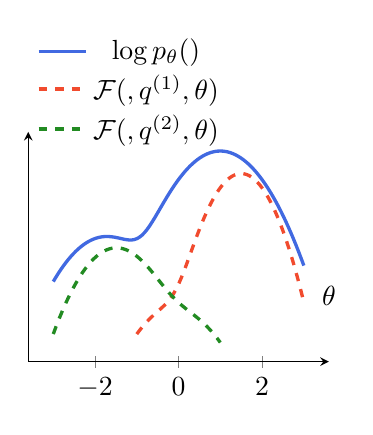
\begin{tikzpicture}
  % Plot settings
  \begin{axis}[
    xlabel=$\theta$, 
    % ylabel={Log likelihood}, 
    axis lines=left, 
    enlargelimits, 
    height=4.5cm, 
    width=5.4cm,
    % legend pos=north west + (0, -0.5cm),
    % legend pos=south,
    yticklabels={},
    ytick=\empty,   % Remove y-axis ticks
    xlabel style={at={(axis description cs:1.0,+0.2)},anchor=south},
    legend style={at={(0,.9)}, anchor=south west, draw=none, fill=none},
    % title={Variational Lower Bound Visualization}
  ]
    
    % True log likelihood (log p(x|theta))
      \addplot[domain=-3:3, samples=100, very thick, RoyalBlue] {ln(2*exp(-(x-1)^2) + 0.1*exp(-(x+1.75)^2))};
    \addlegendentry{$\log p_{\theta}(\rvx)$}

    % Variational lower bound option 1
    \addplot[domain=-1:3., samples=100, very thick, RedOrange, dashed] {ln( 100 * exp(-(x-1.5)^2/0.5) + exp(-(x)^2)) - 4.7};
    \addlegendentry{$\mathcal{F}(\rvx, q^{(1)}, \theta)$}
    % Variational lower bound option 2
    \addplot[domain=-3:1, samples=100, very thick, ForestGreen, dashed] {ln( 10 * exp(-(x+1.5)^2/0.75) + exp(-(x)^2)) - 5.};
    \addlegendentry{$\mathcal{F}(\rvx, q^{(2)}, \theta)$}

    % KL Divergence (gap between the curves)
    % \node at (axis cs:-1, -2) [anchor=north] {KL Divergence};
    % \draw[<->, thick] (axis cs:0, -0.7) -- (axis cs:0, -1.7);

  \end{axis}
\end{tikzpicture}
\caption{Variational lower bound on the loglikelihood.}\label{fig:intro_bound}
\end{marginfigure}
This is a variational lower bound, which is also known as Evidence Lower BOund (ELBO) with \textit{variational} parameter $q$ is visualized in Figure~\ref{fig:intro_bound}. Different variational distributions $q$ will correspond to different lower bounds (e.g. green and red dashed lines in Figure~\ref{fig:intro_bound}), while different values of parameters $\theta$, will correspond to different points on the curve. 
% ELBO can be more or less tight depending on this variational distribution $q$
% to the shifts of the red curve in figure \ref{fig:intro_bound}.

To see how ELBO relates to maximum likelihood and posterior approximation,  consider the following decomposition:
\begin{equation}
\begin{aligned}
    \mathcal{F}(\rvx, q, \theta) &= \E_{q(\rvz)}\log  \frac{p_{\theta}(\rvx,\rvz)}{q(\rvz)} \\
    & = \E_{q(\rvz)}\log  \frac{p_{\theta}(\rvz|\rvx)p_{\theta}(\rvx)}{q(\rvz)} \\
    & = \E_{q(\rvz)}\log  \frac{p_{\theta}(\rvz|\rvx)}{q(\rvz)} +  \log p_{\theta}(\rvx)\\
    & = - \KL{q(\rvz)}{p_{\theta}(\rvz|\rvx)} + \log p_{\theta}(\rvx).\\
\end{aligned}
\end{equation}

This shows that ELBO is equal to the sum of marginal likelihood and the negative KL divergence between the introduced distribution $q(\rvz)$ and the true posterior.
% and makes it clear that the bound is tight when $q(\rvz) = p(\rvz|\rvx)$. 
As \citet{neal1998view} showed,  maximizing ELBO with respect to the distribution $q$ is identical to minimizing the KL divergence. When $q(\rvz) = p(\rvz|\rvx)$ the divergence is zero and the ELBO matches the log-likelihood.
Moreover, \citet{neal1998view} showed that if $\mathcal{F}(\rvx, q, \theta) $ has a maximum at $q^*, \, \theta^*$, then $\log p_{\theta}(\rvx)$ has a maximum at $\theta^*$. That is, ELBO has the same optimum as the maximum likelihood objective. 

\paragraph{Expectation Maximization}
Expectation Maximization Algorithm, also known as a EM-algorithm~\citep{dempster1977maximum} is an iterative algorithm to infer posterior over the latent variables and maximum likelihood estimate of the parameters.
It is usually applied to a class of problems, where $p_{\theta}(\rvz|\rvx)$ is tractable if we fix parameters of the generative model $\theta$. At each iteration, 

\begin{equation}
\begin{aligned}
    \text{\textbf{E-step:  }} &q^{t+1}_n(\rvz) = p_{\theta^t}(\rvz|\rvx_n) = \arg\max_{q_n} \mathcal{F}(\rvx_n, q_n, \theta^t),\;\;\forall n \in \{1\dots N\}\\
    \text{\textbf{M-step:  }} &\theta^{t+1} = \arg\max_{\theta} \E_{p_e(\rvx)}\mathcal{F}(\rvx, q^{t+1}_n, \theta)\\
\end{aligned}
\end{equation}

Expectation step computes posterior distribution given the model parameters from the previous step. Maximization step uses this posterior to optimize the ELBO with respect to parameters $\theta$. From the formulation above, we also see that both steps of the EM-algorithm solve the same optimization problem: maximizing the ELBO.  This observation allows us to generalize this to a wider class of problems where the posterior distribution is not tractable. 

\paragraph{Variational Inference}
When EM-algorithm is intractable, one can still use ELBO as a training objective. 
In order to do that, assume that $q_n$,  variational posterior distribution for a datapoint $\rvx_n$ belongs to a parametric family of distributions defined by parameters $\phi_n$:
\begin{equation}
    \mathcal{Q} = \{q_{\phi_n}(\rvz) | \phi_n \in \Phi\}
\end{equation}
\begin{marginfigure}
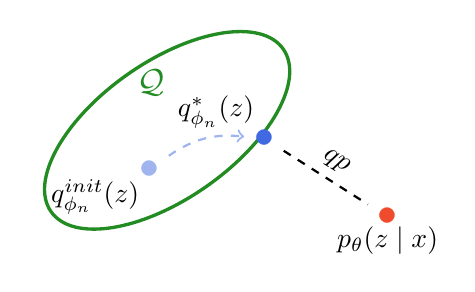
\begin{tikzpicture}
    % Draw the circle representing the variational family
    \draw[very thick, ForestGreen, rotate=35] (0,0) ellipse (1.8cm and 0.87cm) node[above, yshift=0.3cm, xshift=-0.2cm]  {\large$\mathcal{Q}$};
    
    % Point for the true posterior outside the circle
    \node[RedOrange] (trueposterior) at (2.8, -1.1) {\Large$\bullet$};
    \node[below] at (trueposterior) {\normalsize$ p_{\theta}(z \mid x) $};
    
    % Point for the variational distribution on the border of the circle
    \node[RoyalBlue!50] (varfamily_init) at (-0.23, -.5) {\Large$\bullet$};
    \node[below left] at (varfamily_init) {\normalsize $q^{\text{init}}_{\phi_n}(z) $};
    
    \node[RoyalBlue] (varfamily) at (1.23, -.1) {\Large$\bullet$};
    \node[above left] at (varfamily) {\normalsize $q^*_{\phi_n}(z) $};

     % Curvy line between varfamily_init and varfamily
    \draw[thick, RoyalBlue!50, ->, dashed, bend left=20] (varfamily_init) to (varfamily);
    
    % Arrow from variational family to true posterior
    \draw[-, dashed, thick] (varfamily) -- (trueposterior) node[midway, above, sloped] {$\KL{q}{p}$};

    % Labeling the circle
    % \node at (0, -3.5) {Parameter space of \( \lambda \)};

\end{tikzpicture}
\caption{When true posterior distribution lies outside of variational family $\mathcal{Q}$, variational inference return the variational posterioir which is closest to the true one in terms on KL devirgence}
\end{marginfigure}
Note that we will assume that each of $q_{\phi_n}(\rvz)$ is independent of each other, which is known as a \textit{mean-field assumption} and we call $\phi_n$ local parameters, since they are learned separately for each datapoint, as opposed to global parameters $\theta$. The resulting Variational Inference (VI) objective is: 
\begin{equation}
     \mathcal{F}^{VI}(\rvx_n, \phi_n, \theta) =  \E_{q_{\phi_n}(\rvz)}\log  \frac{p_{\theta}(\rvx_n|\rvz)p_{\theta}(\rvz)}{q_{\phi_n}(\rvz)}
\end{equation}
Optimizing this objective function yields $q_{\phi_n}$ from a chosen family of distributions, which is closest to the true posterior in terms of KL-divergence. Analogously to the stochastic version of the gradient descent, stochastic Variational Inference (SVI) was proposed~\citep{hoffman2013stochastic}, where at each iteration only a subset of data is used, and thus only a subset of the local variational parameters $\phi_n$ is updated. 
However, there are still multiple aspects that hinders the scalability of the VI objective. We will now address each of then in detail. 


\paragraph{Amortized Variational Inference}
Even with stochastic VI, having separate local parameters for each datapoint can be very expensive. 
A common way to overcome it is to use amortization. This approach restricts the family of variational distributions even further, assuming that all the $q_n$ are parametrized with the same Neural Network $f_{\phi}$ which maps datapoints $\rvx_n$ to the corresponding parameters of the distribution: 
\begin{equation}
    % \mathcal{Q}_{\text{A}} = \Big\{ q: \prod_n q_{\phi}(\rvz | \rvx_n) \Big\}
    q_{\phi_n}(\rvz) = q_{\phi}(\rvz |\rvx_n).
\end{equation}

The amortized family is a subset of the mean-field variational family and the difference in the quality of the resulting approximations is known as \textit{Amortization Gap}~\citep{cremer2018inference}. It was also shown that a middle ground between AVI and SVI achieves better performance~\citep{kim2018semi}. However, in large scale even a small computational overhead can be detrimental. Therefore, throughout this thesis, we will use amortized variational inference objective:
\begin{equation}\label{eq:intro_avi}
     \mathcal{F}^{AVI}(\rvx, \phi, \theta) =  \E_{q_{\phi}(\rvz)}\log  \frac{p_{\theta}(\rvx|\rvz)p_{\theta}(\rvz)}{q_{\phi}(\rvz|\rvx)}
\end{equation}

\paragraph{Reparametrization trick and doubly stochastic variational inference}
Finally, in order to learn both generative parameters $\theta$ and variational parameters $\phi$, we need to know how to compute the gradients. First, the parametric form of $p_{\theta}(\rvx|\rvz)$, $p_{\theta}(\rvz)$ and $q_{\phi}(\rvz|\rvx)$ allows us to compute the corresponding gradients $\nabla_{\theta}\log p_{\theta}(\rvx|\rvz)$, $\nabla_{\theta}\log p_{\theta}(\rvz)$ and $\nabla_{\theta}\log q_{\phi}(\rvz|\rvx)$ using backpropagation. Given that, the gradient of the Evidence Lower Bound w.r.t $\theta$ is straightforward:
\begin{equation}
    \begin{aligned}
      \nabla_{\theta}\mathcal{F}^{AVI}(\rvx, \phi, \theta) 
      &= \E_{q_{\phi}(\rvz|\rvx)} \nabla_{\theta} \log  \frac{p_{\theta}(\rvx|\rvz)p_{\theta}(\rvz)}{q_{\phi}(\rvz)} \\
      &= \E_{q_{\phi}(\rvz|\rvx)} \nabla_{\theta} \log p_{\theta}(\rvx|\rvz)p_{\theta}(\rvz)
    \end{aligned}
\end{equation}

This quantity can be efficiently computed using Monte-Carlo estimation. In practice, even one-sample estimation works well:

\begin{equation}
    \nabla_{\theta}\mathcal{F}^{AVI}(\rvx, \phi, \theta) \approx \nabla_{\theta} \log p_{\theta}(\rvx|\tilde{\rvz})p_{\theta}(\tilde{\rvz}),\, \tilde{\rvz} \sim q_{\phi}(\rvz|\rvx)
\end{equation}

However, since in Eq.~\ref{eq:intro_avi} the expectation is taken with respect to $q_{\phi}(\rvz|\rvz)$, the gradien computation is less straingtforward. It can be computed using REINFORCE~\citep{williams1992simple} or using the reparametrization trick.  The former uses log-derivative trick to represent the gradient as an expectation; however, it tends to have high variance and is not often used in generative modeling. Reparametrization trick, on other hand, makes use of the change of variable formula and is very widespread. This method was independently proposed for latent variable generative models \cite{kingma2014autoencoding, rezende2014stochastic} and for the Bayesian inference \citep{titsias2014doubly}. 

Consider a random variable $\varepsilon \sim p(\varepsilon)$ and a deterministic transformation $g_{\phi}(\varepsilon, \rvx)$, such that:
\begin{equation}
    \tilde{\rvz} = g_{\phi}(\varepsilon, \rvx)\quad \Rightarrow \quad  \tilde{\rvz} \sim q_{\phi}(\rvz|\rvz)
\end{equation}

We can now use this deterministic transformation to apply change of variable formula to the Eq.~\ref{eq:intro_avi}:
\begin{equation}
\begin{aligned}
     \mathcal{F}^{AVI}(\rvx, \phi, \theta) &=  \E_{p(\varepsilon)}\log  \frac{p_{\theta}(\rvx|\tilde{\rvz})p_{\theta}(\tilde{\rvz})}{q_{\phi}(\tilde{\rvz}|\rvx)},\\
     \text{where}\, \tilde{\rvz} &= g_{\phi}(\varepsilon, \rvx).
\end{aligned}
\end{equation}

This way, the  gradient with respect to $\phi$ can be computed similarly, using Monte Carlo estimate:

\begin{equation}
    \nabla_{\phi}\mathcal{F}^{AVI}(\rvx, \phi, \theta) \approx  \nabla_{\phi}\log  \frac{p_{\theta}(\rvx|\tilde{\rvz})p_{\theta}(\tilde{\rvz})}{q_{\phi}(\tilde{\rvz}|\rvx)},\, \tilde{\rvz} = g_{\phi}(\tilde{\varepsilon}, \rvx)\,\text{ and }\, \tilde{\varepsilon} \sim p(\varepsilon).
\end{equation}

Note, that this approach now has two sources of stochastisity. At each step, we use a subsample of the datapoints (a mini-batch) $\{\rvx_i\}_{i \in \mathcal{M}}$ to estimate the expectation with respect to the empirical distribution $\E_{p_{e}(\rvx)}$ and we sample from the variational posterior (by the mean of the reparametrization trick) to estimate the expectation $\E_{q_{\phi}(\rvz|\rvx)}$. \citet{titsias2014doubly} referred to such method as \textit{Doubly Stochastic Variational Inference} (DDVI). 
However, this term is more common in Bayesian inference rather than in Deep Generative Modeling. Therefore, throughout this thesis, we will mostly refer to it as Amortized Variational Inference with reparametrization trick.


%%%%%%%%%%%%%%%%%%%%%%%%%%%%%%%%%5
% Auxiliarly variables: latent and non-latent
%%%%%%%%%%%%%%%%%%%%%%%%%%%%%%%%%5
\section{Variational Autoencoder}\label{sec:into_deep_generative_models}
%- Latent variable generative models: from PPCA to Diffusion models
%- $$p(x) = p(x|z)p(z)$$
%- Lower dimentional manifold assumption
%- Oldies but goldies: PPCA -> Helmholtz machines / Boltzman machines 
%- Modern heros: Variational Autoencoders, Diffusion Models
%- Amortization and voila, we have variational posterior $$q(z|x)$$


This thesis contributes to the field of Variational Autoencoders (VAE) and Diffusion Models. These are deep generative models with auxiliary variables and are trained with the objectives derived from Amortized Variational Inference. We consider the application of these models to the problem of modeling the distribution on images in different scenarios. The thesis is split into two parts, part~\ref{part:1} focuses on the improved density estimation. Part~\ref{part:2}. on the other hand, takes a closer look at the properties of learned data representations. 

In this section, we focus in more details on the deep Latent Variable model (Eq.~\ref{eq:intro_lvm_def}). We assume  continuous random variable $\rvz$ corresponding to each datapoint. 

First, we discuss the training objective


% Next, there exist several design choces that influnce the 
% This generative model can be interpreted as an infinite mixture model \cite{mattei2018leveraging}. VAEs are trained with the amortized variational inference described in Section~\ref{sec:intro_vi}.

\paragraph{VAE limitations}
\begin{itemize}
    \item Blurry samples \cite{Rybkin2020-je}
    \item Posterior Collapse \\
    \cite{kingma2016improved} proposed free bits to solve posterior collapse    
    \item Holes in the latent space
\end{itemize}



% Here \cite{mattei2018leveraging}, this interpretation allowed to obtain an upper bound on the likelihood. 
\subsection{ELBO as a training objective}

Consider the Evidence Lower Bounds that is used to train VAEs. There are multiple ways to re-write this objective which give rise to different intuition regarding the VAE model. We start from the following decomposition:
\begin{equation}\label{eq:intro_elbo_again}
\mathcal{L}(\theta, \phi) = \E_{p_e(\rvx)}\Big[ \underbrace{\E_{q_{\phi}(\rvz|\rvx)} \log p_{\theta}(\rvx| \rvz)}_{\text{Reconstruction Loss}} - \underbrace{\KL{q_{\phi}(\rvz|\rvx)}{p_{\theta}(\rvz)}}_{\text{KL term}} \Big]% \rightarrow \max_{\phi, \theta}
\end{equation}

\paragraph{Reconstruction Loss}
\marginnote[0\baselineskip]{It is common to call the variational posterior \textit{encoder} and the conditional likelihood \textit{decoder}. Thus, when both distributions are learned together, the resulting model can be seen as a probabilistic version of the AutoEcoder.}
The first part of ElBO in Eq.~\ref{eq:intro_elbo_again} ensures that the model is able to reconstruct the input $\rvx$. If we consider it's a Monte-Carlo estimator for a single datapoint, it is computed by first sampling $\tilde{\rvz}_n$ for a given datapoint from the variational posterior and then computing the conditional log-likelihood using this sample:


\begin{equation}
\begin{aligned}
    \tilde{\rvz}_n &\sim q_{\phi}(\cdot|\rvx_n), \\
    \text{Re}(\rvx_n) &= \log p_{\theta}(\rvx_n|\tilde{\rvz}_n).
    \end{aligned}
\end{equation}
In other words, we \textit{encode} data into the latent space and then \textit{reconstruct} it. 

\paragraph{KL term}

The second tern can be seen as a regularizer. It ensures that the variational posterior is close to the distribution $p_{\theta}(\rvz)$, which is usually called \textit{prior}\footnote{
The name \textit{prior} often suggests that this distribution is given to us \textit{apriori}. However, we will often employ an approach in which the distribution $p_{\theta}(\rvz)$ has learnable parameters and is learned together with the conditioanl likelihood. This is analogous to Empirical Bayes \cite{wang2019comment} approach, where prior is estimated from the data. 
}. 
Thus, after a model is trained, one can sample latent code from the prior \textit{uncoditionally} and then decode using the conditional likelihood. 

\paragraph{Constrained Optimization Framework}
One can also consider ELBO objective form the constrained optimization point of view \citep{higgins2017beta, rezende2018taming}. \citet{higgins2017beta} introduce $\beta$-VAE, where additional hyperparameters $\beta$ it used to re-weight the KL-term in Eq.~\ref{eq:intro_elbo_again}. A more general approach is introduces by \citet{rezende2018taming}, where the authors 


\todo[inline]{fixing the broken ELBO}

Let us introduce an \textit{aggregated posterior} which is defined as a variational posterior averaged over the whole dataset: $q_{\phi}(\rvz) = \E_{p_{e}(\rvx)}q_{\phi}(\rvz|\rvx)$.
Following \citet{hoffman2016elbo} we can use the aggregated posterior to further study the average KL:

\begin{equation}\label{eq:intro_elbo_vamp}
\begin{aligned}
&\E_{p_e(\rvx)} \KL{q_{\phi}(\rvz|\rvx)}{p_{\theta}(\rvz)} \\
&\; = \E_{p_e(\rvx)} \int q_{\phi}(\rvz|\rvx) \log \frac{q_{\phi}(\rvz|\rvx)}{p_{\theta}(\rvz)}\frac{q_{\phi}(\rvz)}{q_{\phi}(\rvz)}d\rvz \\
&\; = \E_{p_e(\rvx)} \int q_{\phi}(\rvz|\rvx) \log \frac{q_{\phi}(\rvz)}{p_{\theta}(\rvz)}d\rvz
+ \E_{p_e(\rvx)} \int q_{\phi}(\rvz|\rvx) \log \frac{q_{\phi}(\rvz|\rvx)}{q_{\phi}(\rvz)}d\rvz\\
&\; =  \int\underbrace{\left( \int p_{e}(\rvx) q_{\phi}(\rvz|\rvx)d\rvx\right)}_{q_{\phi}(\rvz)} \log \frac{q_{\phi}(\rvz)}{p_{\theta}(\rvz)}d\rvz
+ \E_{p_e(\rvx)} \KL{q_{\phi}(\rvz|\rvx)}{q_{\phi}(\rvz)} \\
&\; =  \KL{q_{\phi}(\rvz)}{p_{\theta}(\rvz)}
+ \E_{p_e(\rvx)} \KL{q_{\phi}(\rvz|\rvx)}{q_{\phi}(\rvz)} \\
\end{aligned}
\end{equation}

This decomposition highlights the importance of multimodal priors. Note that the prior distirbution is only present in the first term: KL-divergence between the aggregated posterior and prior. Therefore, the prior that minimizes the ELBO is equal to the aggregated posterior. The later is the \textit{mixture} of encoders~\footnote{It is vary common to use Gaussian distribution for $q_{\phi}(\rvz|\rvx)$. In this case aggregated posterior is a Gaussian mixture.}



% Note that $q_{\phi}(\rvz)$ is a mixture of the variational posteriors. That is, in the case of Gaussian $q_{\phi}(\rvz|\rvx)$ a mixture of $N$ gaussians. 
% \todo[inline]{the importance of multimodal prior distribution}
 

Auxiliary Deep Generative Models \cite{maaloe2016auxiliary}



\subsection{Conditional Likelihood}


\paragraph{Modeling pixel values}
Images are usually considered as continious objects, where each pixel is assigned with the corresponding intensity $\nu$. 
However, the observed value $\rvx$ is usually discretized (e.g. intensity rounded to the nearest 8-bit representation). 
Therefore, using continuous distribution might be sub-optimal.
One option in this case would be to use Categorical distribution with 256 possible values for each pixel (in case of the 8-bit representation). However, this will ignore the fact that the nearby pixel values are correlated. 
Instead, a common approach is to model the pixel intensity as a continuous random variable and then discretize its distribution to calculate the actual likelihood. 
% Generally, there are two ways to implement this discretization which we will consider now. 

We will assume that all pixel across spacial and channel dimensions are conditionally independent:
\begin{equation}
    p_{\theta}(\rvx|\rvz) = \prod_i p_{\theta}(\rvx_i|\rvz),\\
    p_{\theta}(\rvx_i|\rvz) = \sum_{k} P_{\theta}(\rvx_i = k|\rvz)
\end{equation}

\begin{marginfigure}
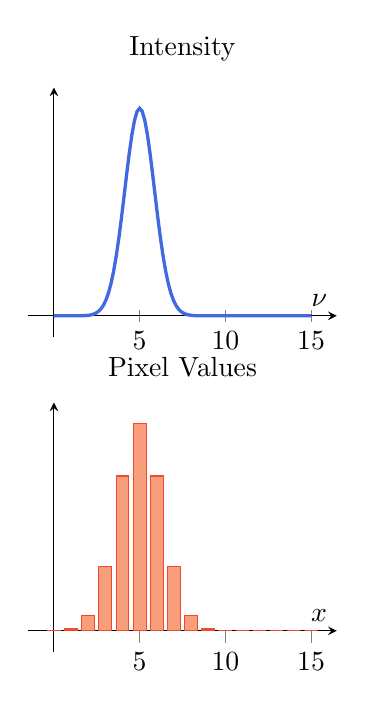
\begin{tikzpicture}
  \begin{axis}[
  name=plot1,
    domain=0:15, 
    samples=100, 
    xlabel=$\nu$, 
    % ylabel={$f(x)$}, 
    axis lines=middle, 
    enlargelimits, 
    title={Intensity}, 
    % height=4cm, 
    width=5.5cm,
    yticklabels={},
    ytick=\empty,   % Remove y-axis ticks
  ]
    \addplot[very thick, RoyalBlue] {1/(sqrt(2*pi*0.75)) *  exp(-0.5 * (x-5)^2/0.75};
  \end{axis}

  \begin{axis}[
  name=plot2,
  at={(0,-4cm)},
    % domain=0:15, 
    % samples=100, 
    xlabel=$x$, 
    % ylabel={$f(x)$}, 
    axis lines=middle, 
    enlargelimits, 
    title={Pixel Values}, 
    % height=4cm, 
    width=5.5cm,
    ybar,
    bar width=0.75,
    yticklabels={},
    ytick=\empty,   % Remove y-axis ticks
  ]
   % Discrete points from the Gaussian distribution
    \addplot[RedOrange, fill=RedOrange!50] coordinates {
    (0, 1.5542e-04) (1, 2.6974e-03) (2, 2.2067e-02) (3, 9.4961e-02) (4, 2.2761e-01) 
    (5, 3.0502e-01) (6, 2.2761e-01) (7, 9.4961e-02) (8, 2.2067e-02) (9, 2.6974e-03)
    (10, 1.5211e-04) (11, 3.3379e-06) (12, 0) (13, 0) (14, 0) (15, 0)
    };
    % \addplot[blue, thick] {1/(sqrt(2*pi*0.5)) *  exp(-0.5 * (x-5)^2/0.5};
  \end{axis}
    % Arrow from the first plot to the second plot
  % \draw[->, thick](plot1.south east) -- (plot2.north west) node[midway, right] {};

\end{tikzpicture}
\end{marginfigure}

Where $\rvx_i$ is a single pixel of an image in an 8-bit representation and $k$ is a particular pixel value. 
Assume that pixel intensity has a continuous distribution with the probability density function $f_{\nu}$ and cumulative distribution function (CDF) $F_{\nu}$. We can discritize it in two ways. 

The first option is to split the support of the intensity random variable into bins and copmute probability of each bin via integration:
\begin{equation}
\begin{aligned}
    &P_{\theta}(\rvx_i = k|\rvz) = \int_{\delta_{-}(\rvx_i)}^{\delta_{+}(\rvx_i)} f_{\nu}(\nu|\rvz)d\nu,\\
    &\delta_{-}(\rvx_i) =
    \begin{cases}
        \infty,\quad &\text{if } \rvx_i = 0\\
        \rvx_i + \frac12,\quad&\text{otherwise}
    \end{cases},  \quad
    \delta_{+}(\rvx_i) =
    \begin{cases}
        -\infty,\quad &\text{if } \rvx_i = 255\\
        \rvx_i - \frac12,\quad&\text{otherwise}
    \end{cases} 
\end{aligned}
\end{equation}

Assuming that we know the CDF of the intensity, we ca compute the value of the integral:
\begin{equation}
    P_{\theta}(\rvx_i = k|\rvz) =\begin{cases}
    F_{\nu}(\rvx_i + \frac{1}{2}) - F_{\nu}(\rvx_i - \frac{1}{2}),\quad &\text{if } k \in (1, \dots, 254) \\
    F_{\nu}(\rvx_i + \frac{1}{2}) - 0,\quad &\text{if } k = 0 \\
    1 - F_{\nu}(\rvx_i - \frac{1}{2}),\quad &\text{if } k = 255 \\
    \end{cases}
\end{equation}
It is convenient to use logistic distribution~\cite{kingma2016improved}, as it's CDF can be easily computed:
\begin{equation}
    F^{\text{logistic}}(x; \mu, \sigma) = \frac{1}{1 + \exp (- \frac{x - \mu}{\sigma})}
\end{equation}

\citet{salimans2016improved} proposed to use a mixture of discretized logistic distributions to improve the flexibility the distribution. It was later used in deep hierarchical VAEs \citep{vahdat2020nvae, Child2020-ze}.

The second option is to re-normalize the probability of each bin:
\begin{equation}
\begin{aligned}
    P_{\theta}(\rvx_i = k|\rvz) = \frac{f_{\nu}(k|\rvz)}{\sum_{i=0}^K f_{\nu}(i|\rvz)}
\end{aligned}
\end{equation}

Note that in this case, we only need to know the PDF of the pixel intensity up to a moralization constant. For example, we can assume gaussian distribution of the pixel intensity and re-normalize using softmax:

\begin{equation}
\begin{aligned}
    P_{\theta}(\rvx_i = k|\rvz) = \frac{\exp\left(-0.5 \frac{\left(\mu(\rvz) - k\right)^2}{\sigma^2(\rvz)}\right)}{\sum_{i=0}^K \exp\left(-0.5 \frac{\left(\mu(\rvz) - i\right)^2}{\sigma^2(\rvz)}\right)}
\end{aligned}
\end{equation}

There is one imaportant difference between two apporaches. The first discretization option assigns higher probability to the pixels 0 and 255. \citet{salimans2016improved} motivated this by the empirical observation that these values have higer appearence in real data. However, this has an effect that in order to learn confident prediction of the pixel values that are close to 0 or 255, the model has to learn a smaller variance of the intensity. Re-normaliation, on the other hand, devide all bins by the same normalization constant.

% So the experiments
% Make the variance separatele learned parameter, initilize at zero. 

% Likelihood Options:
    % Gaussian tail CDF
    % Logistic tail CDF
    % Gaussian softmax

% Variance Otions:
    % No Limit
    % Clip 1/sigma at 1000
    % Clip 1/sigma at 500











\subsection{Learnable Priors}


Concerning the priors in VAEs. Starting from the standard Gaussian, we can talk a lot about using different distributions. 

The learnable prior adapts to the data, the first example being the flow-based prior and the second VampPrior.
Then we talk about VampPrior and how it was then used by the field a lot. 
Maybe, how it was combined with the Constrained Optimization framework

If prior is data-dependent it can be used to store information and avoid catastrophic forgetting in continual learning.



\begin{quote}
	How \marginnote[-0\baselineskip]{Research Question 1} to adjust optimal prior to train VAEs in continual learning?
\end{quote}
This research question is addressed in Chapter~\ref{chap:boovae}.

\subsection{Hierarchical VAEs}
Next, we switch to heirarchical VAEs. Here we say that we can decompose latent variables into groups or stochastic layers and define a prior in the autoregressive way. This allows to get a very expressive latent distribution. However, they \textbf{can be hard to train} and \textbf{tend to have a lot of inactive units}.


\begin{quote}
	How \marginnote[-0.75\baselineskip]{Research Question 2} to approximate the optimal prior for hierarchical VAEs in a scalable way and improve latent space utilization?
\end{quote}
This research question in addressed in Chapter~\ref{chap:dvp}.

\subsection{Is Variational Posterior Distribution an Encoder?}
How latent variabel model resembles autoencdoer and why variational posterioir is called an encode sometimes

How can VAEs be used to learn latent representation. 

If we do, then we want some properties of those latent representations. 

For example, we want those latent representations to be robust to adversarial attacks. 
\begin{quote}
	How \marginnote[-0.75\baselineskip]{Research Question 3} to make latent representations robust to adversarial attacks?
\end{quote}
This research question is addressed in Chapter~\ref{chap:adv_att}.


Therefore, we want to be aware of the properties latent spaces possess or want to be able to impose properties we downstream tasks require. For example, one may need to preserve the symmetries of the data when obtaining its latent representation. 


\paragraph{Compressed Sensing}
\begin{quote}
	How \marginnote[-0.75\baselineskip]{Research Question 4} to train VAE with the equivariant latent space and use it as a prior for compressed sensing with unknown rotation.
\end{quote}
This research question is addressed in Chapter~\ref{chap:eqvae}.


\section{Non-latent Auxiliary Variables in Generative Models}
In the previous section, auxillary variables were unobserved and we had to infer posterior disitrobution from the data. Another option could be when auxillary variables are observed or we know their conditional distribution. For example, diffusion based generative models introduce $T$ auxillary variables which constitute noise versions of the input $\rvx$ with different level of noise. We then apply maximum likelihood over the joint model:
\begin{equation}
p_{\theta}(\rvx, \rvz_1, \dots, \rvz_T)
\end{equation}

Interestingly, the MLE objective above is nothing mode than a special case of the ELBO (Eq.~\ref{eq:intro_elbo}), where variational posterior is not learnable. This connection between diffusion and latent variable models was observed by \citet{huang2021variational, kingma2021variational, tzen2019neural}.

The most popular way to define such non-latent auxilary variable is by using diffusion process, which gradually destroys the initial signal by adding more and mode noise to it. Then, generative model is essentially is trained to "undo" the harm. Such generative models are called Denoising Diffusion Generative Model.

\begin{quote}
	How \marginnote[-0.75\baselineskip]{Research Question 5} to decouple denoising and generative abilities of the diffusion generative models
\end{quote}
This research question is addressed in Chapter~\ref{chap:daed}.


% \newpage
\section{Dissertation Structure and Contributions}
In the process of answering the research questions above, we have contributed to different aspects of generative modeling. In Table \ref{tab:papers_and_contributions} we provide the matrix of conrtibutions, so that the reader interested in a particular aspect can refer to the 
\begin{table}[!ht]
	\caption[][\baselineskip]{Contributions to Different Aspects of Generative Modeling .}
	\label{tab:papers_and_contributions}
	\begin{center}
%		\resizebox{\textwidth}{!}{
			\begin{tabular}{ll|cccc}
				\toprule
				& &         & Downstream & Latent                & Architecture \\
				& & Prior & Application  & Space Properties &                      \\ \midrule
				\multirow{2}{*}{\STAB{\rotatebox[origin=c]{90}{Part 1}}}
				& Chapter \ref{chap:boovae} & $\checkmark$ & $\checkmark$ & \\
				& Chapter \ref{chap:dvp} & $\checkmark$ & & & $\checkmark$\\ \midrule
				\multirow{3}{*}{\STAB{\rotatebox[origin=c]{90}{Part 2}}}
				& Chapter \ref{chap:eqvae}&  &$\checkmark$ & $\checkmark$ & $\checkmark$\\
				& Chapter \ref{chap:adv_att} & &$\checkmark$ & $\checkmark$ &\\
				& Chapter \ref{chap:daed} &  & & $\checkmark$ &\\
				 \midrule
				\bottomrule
				% \end{tabularx}
			\end{tabular}
%		}
	\end{center}
	\vspace*{\baselineskip}
\end{table}
%\section{Research Questions}
%
%\begin{enumerate}
%\item Approximate optimal prior improves the VAE performance. How to adjust it to be applicable to continual learning setting and be scalable to deep hierarchical VAEs?
%\item How to make sure that latent representation exhibit predictable performance under certain input transformations, such as specifically constrcuted noise or action of the symmetry group?
%\item  What are the banifits of using VAEs as generative prior in continual learning and compressed sensing
%\item  Can we decouple denoising and generative functions of the diffusion latent space?
%\item  How to improve latent space utilization in deep hierarchical VAEs?
%\end{enumerate}

\paragraph{How to read this dissertation}
Each chapter in this dissertation is based on one or more published papers.
We have chosen to keep paper consistent with the original publication, which allows reading each chapter as independent unit. 
Each paper is accompanied with Appendix, which is located at the end of the dissertation.


